% AER E 361 Mission Report Template
% Spring 2023
% Template created by Yiqi Liang and Professor Matthew Nelson

% Document Configuration DO NOT CHANGE
\documentclass[12 pt]{article}
% --------------------LaTeX Packages---------------------------------
% The following are packages that are used in this report.
% DO NOT CHANGE ANY OF THE FOLLOWING OR YOUR REPORT WILL NOT COMPILE
% -------------------------------------------------------------------

\usepackage{hyperref}
\usepackage{parskip}
\usepackage{titlesec}
\usepackage{titling}
\usepackage{graphicx}
\usepackage{graphviz}
\usepackage[T1]{fontenc}
\usepackage{titlesec, blindtext, color} %for LessIsMore style
\usepackage{tcolorbox} %for references box
\usepackage[hmargin=1in,vmargin=1in]{geometry} % use 1 inch margins
\usepackage{float}
\usepackage{tikz}
\usepackage{svg} % Allows for SVG Vector graphics
\usepackage{textcomp, gensymb} %for degree symbol
\hypersetup{
	colorlinks=true,
	linkcolor=blue,
	urlcolor=cyan,
}
\usepackage{biblatex}
\addbibresource{lab-report-bib.bib}
\usepackage{amsmath}
\usepackage{listings}
\usepackage{multicol}
\usepackage{array}

\usepackage{hologo} %KYR: for \BibTeX
%\usepackage{algpseudocode}
%\usepackage{algorithm}
% This configures items for code listings in the document
\usepackage{xcolor}

\usepackage{fancyhdr} % Headers/Footers
\usepackage{siunitx} % SI units
\usepackage{csquotes} % Display Quote
\usepackage{microtype} % Better line breaks

\definecolor{commentsColor}{rgb}{0.497495, 0.497587, 0.497464}
\definecolor{keywordsColor}{rgb}{0.000000, 0.000000, 0.635294}
\definecolor{stringColor}{rgb}{0.558215, 0.000000, 0.135316}
\definecolor{mygreen}{rgb}{0,0.6,0}
\definecolor{mygray}{rgb}{0.5,0.5,0.5}
\definecolor{mymauve}{rgb}{0.58,0,0.82}

\lstdefinestyle{customc}{
  belowcaptionskip=1\baselineskip,
  breaklines=true,
  frame=L,
  xleftmargin=\parindent,
  language=C,
  showstringspaces=false,
  basicstyle=\footnotesize\ttfamily,
  keywordstyle=\bfseries\color{green!40!black},
  commentstyle=\itshape\color{purple!40!black},
  identifierstyle=\color{blue},
  stringstyle=\color{orange},
 }

 \lstset{ %
  backgroundcolor=\color{white},   % choose the background color; you must add \usepackage{color} or \usepackage{xcolor}
  basicstyle=\footnotesize,        % the size of the fonts that are used for the code
  breakatwhitespace=false,         % sets if automatic breaks should only happen at whitespace
  breaklines=true,                 % sets automatic line breaking
  captionpos=b,                    % sets the caption-position to bottom
  commentstyle=\color{commentsColor}\textit,    % comment style
  deletekeywords={...},            % if you want to delete keywords from the given language
  escapeinside={\%*}{*)},          % if you want to add LaTeX within your code
  extendedchars=true,              % lets you use non-ASCII characters; for 8-bits encodings only, does not work with UTF-8
  frame=tb,	                   	   % adds a frame around the code
  keepspaces=true,                 % keeps spaces in text, useful for keeping indentation of code (possibly needs columns=flexible)
  keywordstyle=\color{keywordsColor}\bfseries,       % keyword style
  language=Python,                 % the language of the code (can be overrided per snippet)
  otherkeywords={*,...},           % if you want to add more keywords to the set
  numbers=left,                    % where to put the line-numbers; possible values are (none, left, right)
  numbersep=8pt,                   % how far the line-numbers are from the code
  numberstyle=\tiny\color{commentsColor}, % the style that is used for the line-numbers
  rulecolor=\color{black},         % if not set, the frame-color may be changed on line-breaks within not-black text (e.g. comments (green here))
  showspaces=false,                % show spaces everywhere adding particular underscores; it overrides 'showstringspaces'
  showstringspaces=false,          % underline spaces within strings only
  showtabs=false,                  % show tabs within strings adding particular underscores
  stepnumber=1,                    % the step between two line-numbers. If it's 1, each line will be numbered
  stringstyle=\color{stringColor}, % string literal style
  tabsize=2,	                   % sets default tabsize to 2 spaces
  title=\lstname,                  % show the filename of files included with \lstinputlisting; also try caption instead of title
  columns=fixed                    % Using fixed column width (for e.g. nice alignment)
}

\lstdefinestyle{customasm}{
  belowcaptionskip=1\baselineskip,
  frame=L,
  xleftmargin=\parindent,
  language=[x86masm]Assembler,
  basicstyle=\footnotesize\ttfamily,
  commentstyle=\itshape\color{purple!40!black},
}

\lstset{escapechar=@,style=customc}

\titlelabel{\thetitle.\quad}

% From here on out you can start editing your document
\newcommand{\subtitle}[1]{%
  \posttitle{%
    \par\end{center}
    \begin{center}\LARGE#1\end{center}
    \vskip0.5em}%
}

\title{\textbf{Iowa State University
\\{\Large Aerospace Engineering}}}
\subtitle{AER E 322 Lab 2\\
		  Stress Concentration}
\author{Matthew Mehrtens, Peter Mikolitis, and Natsuki Oda}

\newcommand{\etal}{\textit{et al}., }
\newcommand{\ie}{\textit{i}.\textit{e}., }
\newcommand{\eg}{\textit{e}.\textit{g}., }

% Define the headers and footers
\setlength{\headheight}{70.63135pt}
\geometry{head=70.63135pt, includehead=true, includefoot=true}
\pagestyle{fancy}
\fancyhead{}\fancyfoot{} % clears the headers/footers
\fancyhead[L]{\textbf{AER E 322}}
\fancyhead[C]{\textbf{Aerospace Structures Laboratory Summary}\\
			  \textbf{Lab 2 Stress Concentration}\\
			  Section 4 Group 2\\
			  Matthew Mehrtens, Peter Mikolitis, and Natsuki Oda\\
			  \today}
\fancyhead[R]{\textbf{Spring 2023}}
\fancyfoot[C]{\thepage}

\begin{document}
\maketitle
\tableofcontents
\section{Introduction} \label{introduction}
This lab will demonstrate how internal stresses change due to stress concentrators using a special material with photoelastic properties. To view the stresses, we will use a special tool called a light-field circular polariscope (Figure \ref{fig:apparatus}). The light-field circular polariscope utilizes two polarized sheets that visualize the internal stresses, specifically the difference between the principal stresses, $\sigma_{p1}-\sigma_{p2}$. To examine the effects of different types of stress concentrators, we will test three different samples: a notched sample, an arched sample, and a sample with a hole.

\begin{figure}[htbp]
\centering
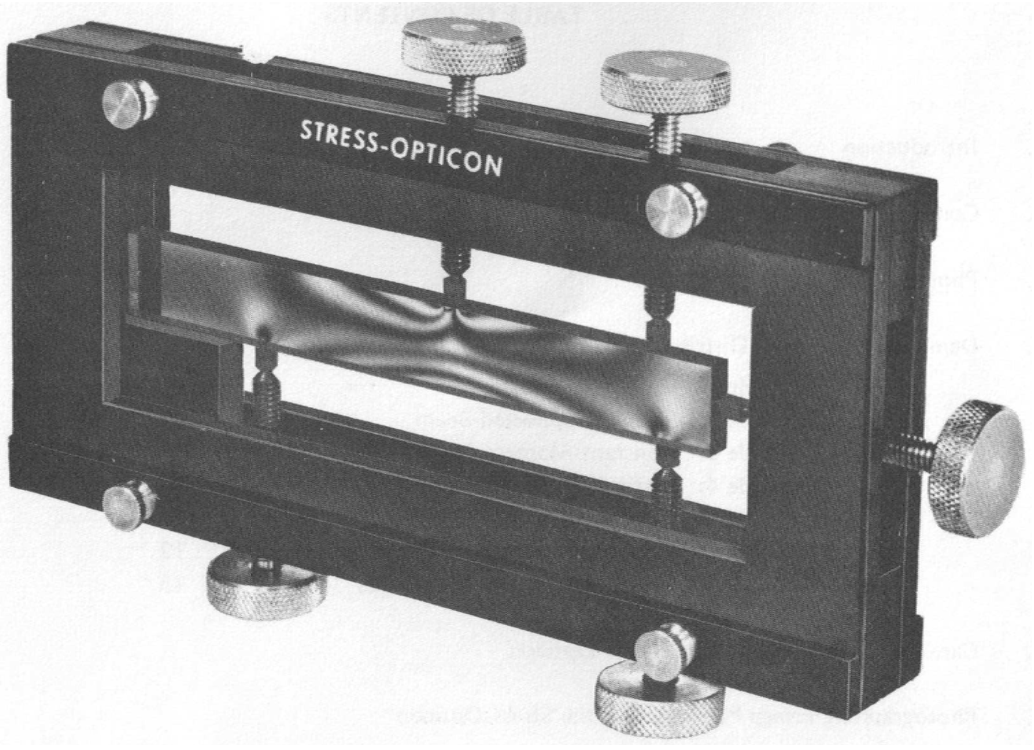
\includegraphics[width=4in]{images/Apparatus}
\caption{The light-field circular polariscope. Image from the Lecture 2 Notes. Copyright 2023 by Thomas Chiou.}
\label{fig:apparatus}
\end{figure}

Using MATLAB, we will analyze the stress equations for a sample with a hole in it. Our MATLAB scripts will reveal the maxima and minima for the three different types of internal stresses: $\sigma_r$, $\sigma_\theta$, and $\sigma_{r\theta}$. Additionally, we will plot the different stress distributions and the difference between the principal stresses. We will compare the theoretical plot of the principal stress difference with the pictures gathered from the experiment.

\section{Objectives} \label{objectives}
To observe how internal stress changes due to stress discontinuities, also known as stress concentrators, and to analyze theoretical internal stresses due to stress concentrators using MATLAB. An example of stress concentrators is shown in Figure \ref{fig:stress_concentrators}.

\begin{figure}[htbp]
\centering
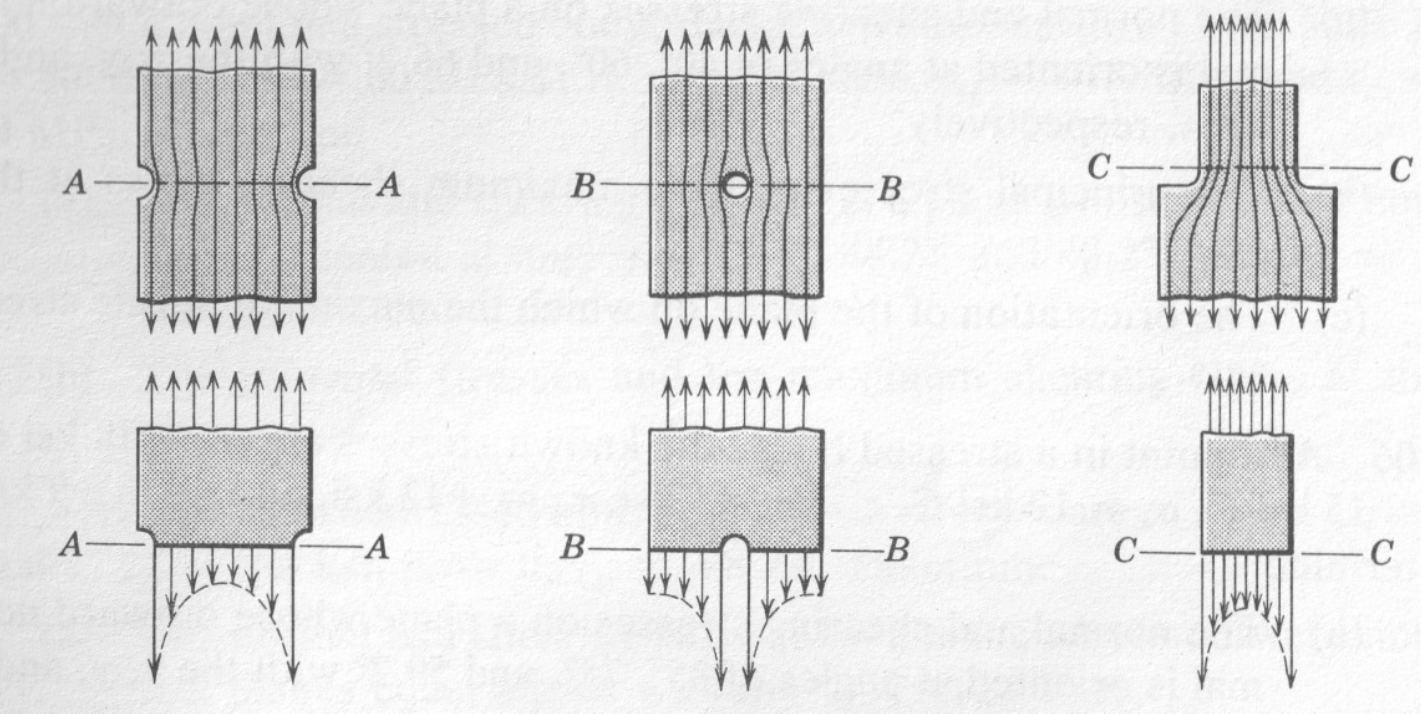
\includegraphics[width=6in]{images/Stress_Concentrators}
\caption{An example of stress discontinuities or concentrators. Image from A. Higdon et al., \textit{Mechanics of Materials}, 4th ed, 1985.}
\label{fig:stress_concentrators}
\end{figure}

\section{Hypothesis} \label{hypothesis}
Due to the photoelastic nature of the material and the polarized sheets, we will be able to clearly photograph the internal stress patterns around the stress concentrators. The difference between the principal stresses will be higher closer to the edges of the discontinuities.

\section{Work Assignments} \label{work_assignments}
Refer to Table \ref{table:work_assignments} for the distribution of work during this lab.

\begin{table}[!htbp]
\caption{Work assignments for AER E 322 Lab 2.}
\begin{center}
	\begin{tabular}{| c | c | c | c |}
		\hline
		\multicolumn{1}{| c |}{\textbf{Task}} & \textbf{Matthew} & \textbf{Peter} & \textbf{Natsuki} \\
		\hline
		\multicolumn{4}{| c |}{\textit{Lab Work}} \\
		\hline
		Date Recording & X & X & X \\
		\hline
		Exp. Setup & X & X & X \\
		\hline
		Exp. Work & X & X & X \\
		\hline
		Exp. Clean-Up & X & X & X \\
		\hline
		\multicolumn{4}{| c |}{\textit{Post Lab}} \\
		\hline
		Question 1 & X & & \\
		\hline
		Question 2 & X & X & \\
		\hline
		Question 3 & X & X & X \\ 
		\hline
		\multicolumn{4}{| c |}{\textit{Report}} \\
		\hline
		Introduction & & X & \\
		\hline
		Objectives & & X & \\
		\hline
		Hypothesis & & X & \\
		\hline
		Materials & & X & \\
		\hline
		Apparatus & & & X \\
		\hline
		Procedures & & & X \\
		\hline
		Data & X & X & X \\
		\hline
		Analysis & X & X & X \\
		\hline
		Conclusion & X & X & \\
		\hline
		Revisions & X & X & \\
		\hline
		Editing & X & & \\
		\hline
	\end{tabular}
\end{center}
\label{table:work_assignments}
\end{table}

\section{Materials} \label{materials}
% TODO

\section{Apparatus} \label{apparatus}
% TODO

\section{Procedures} \label{procedures}
% TODO

\section{Data} \label{data}
% TODO

\section{Analysis} \label{analysis}
% TODO

\section{Conclusion} \label{conclusion-section}
% TODO

\end{document}
